\chapter{Proposed Methodology and Mathematical Framework}
\label{chap:3}


\newpage

\begin{figure}[H]
    \centering
    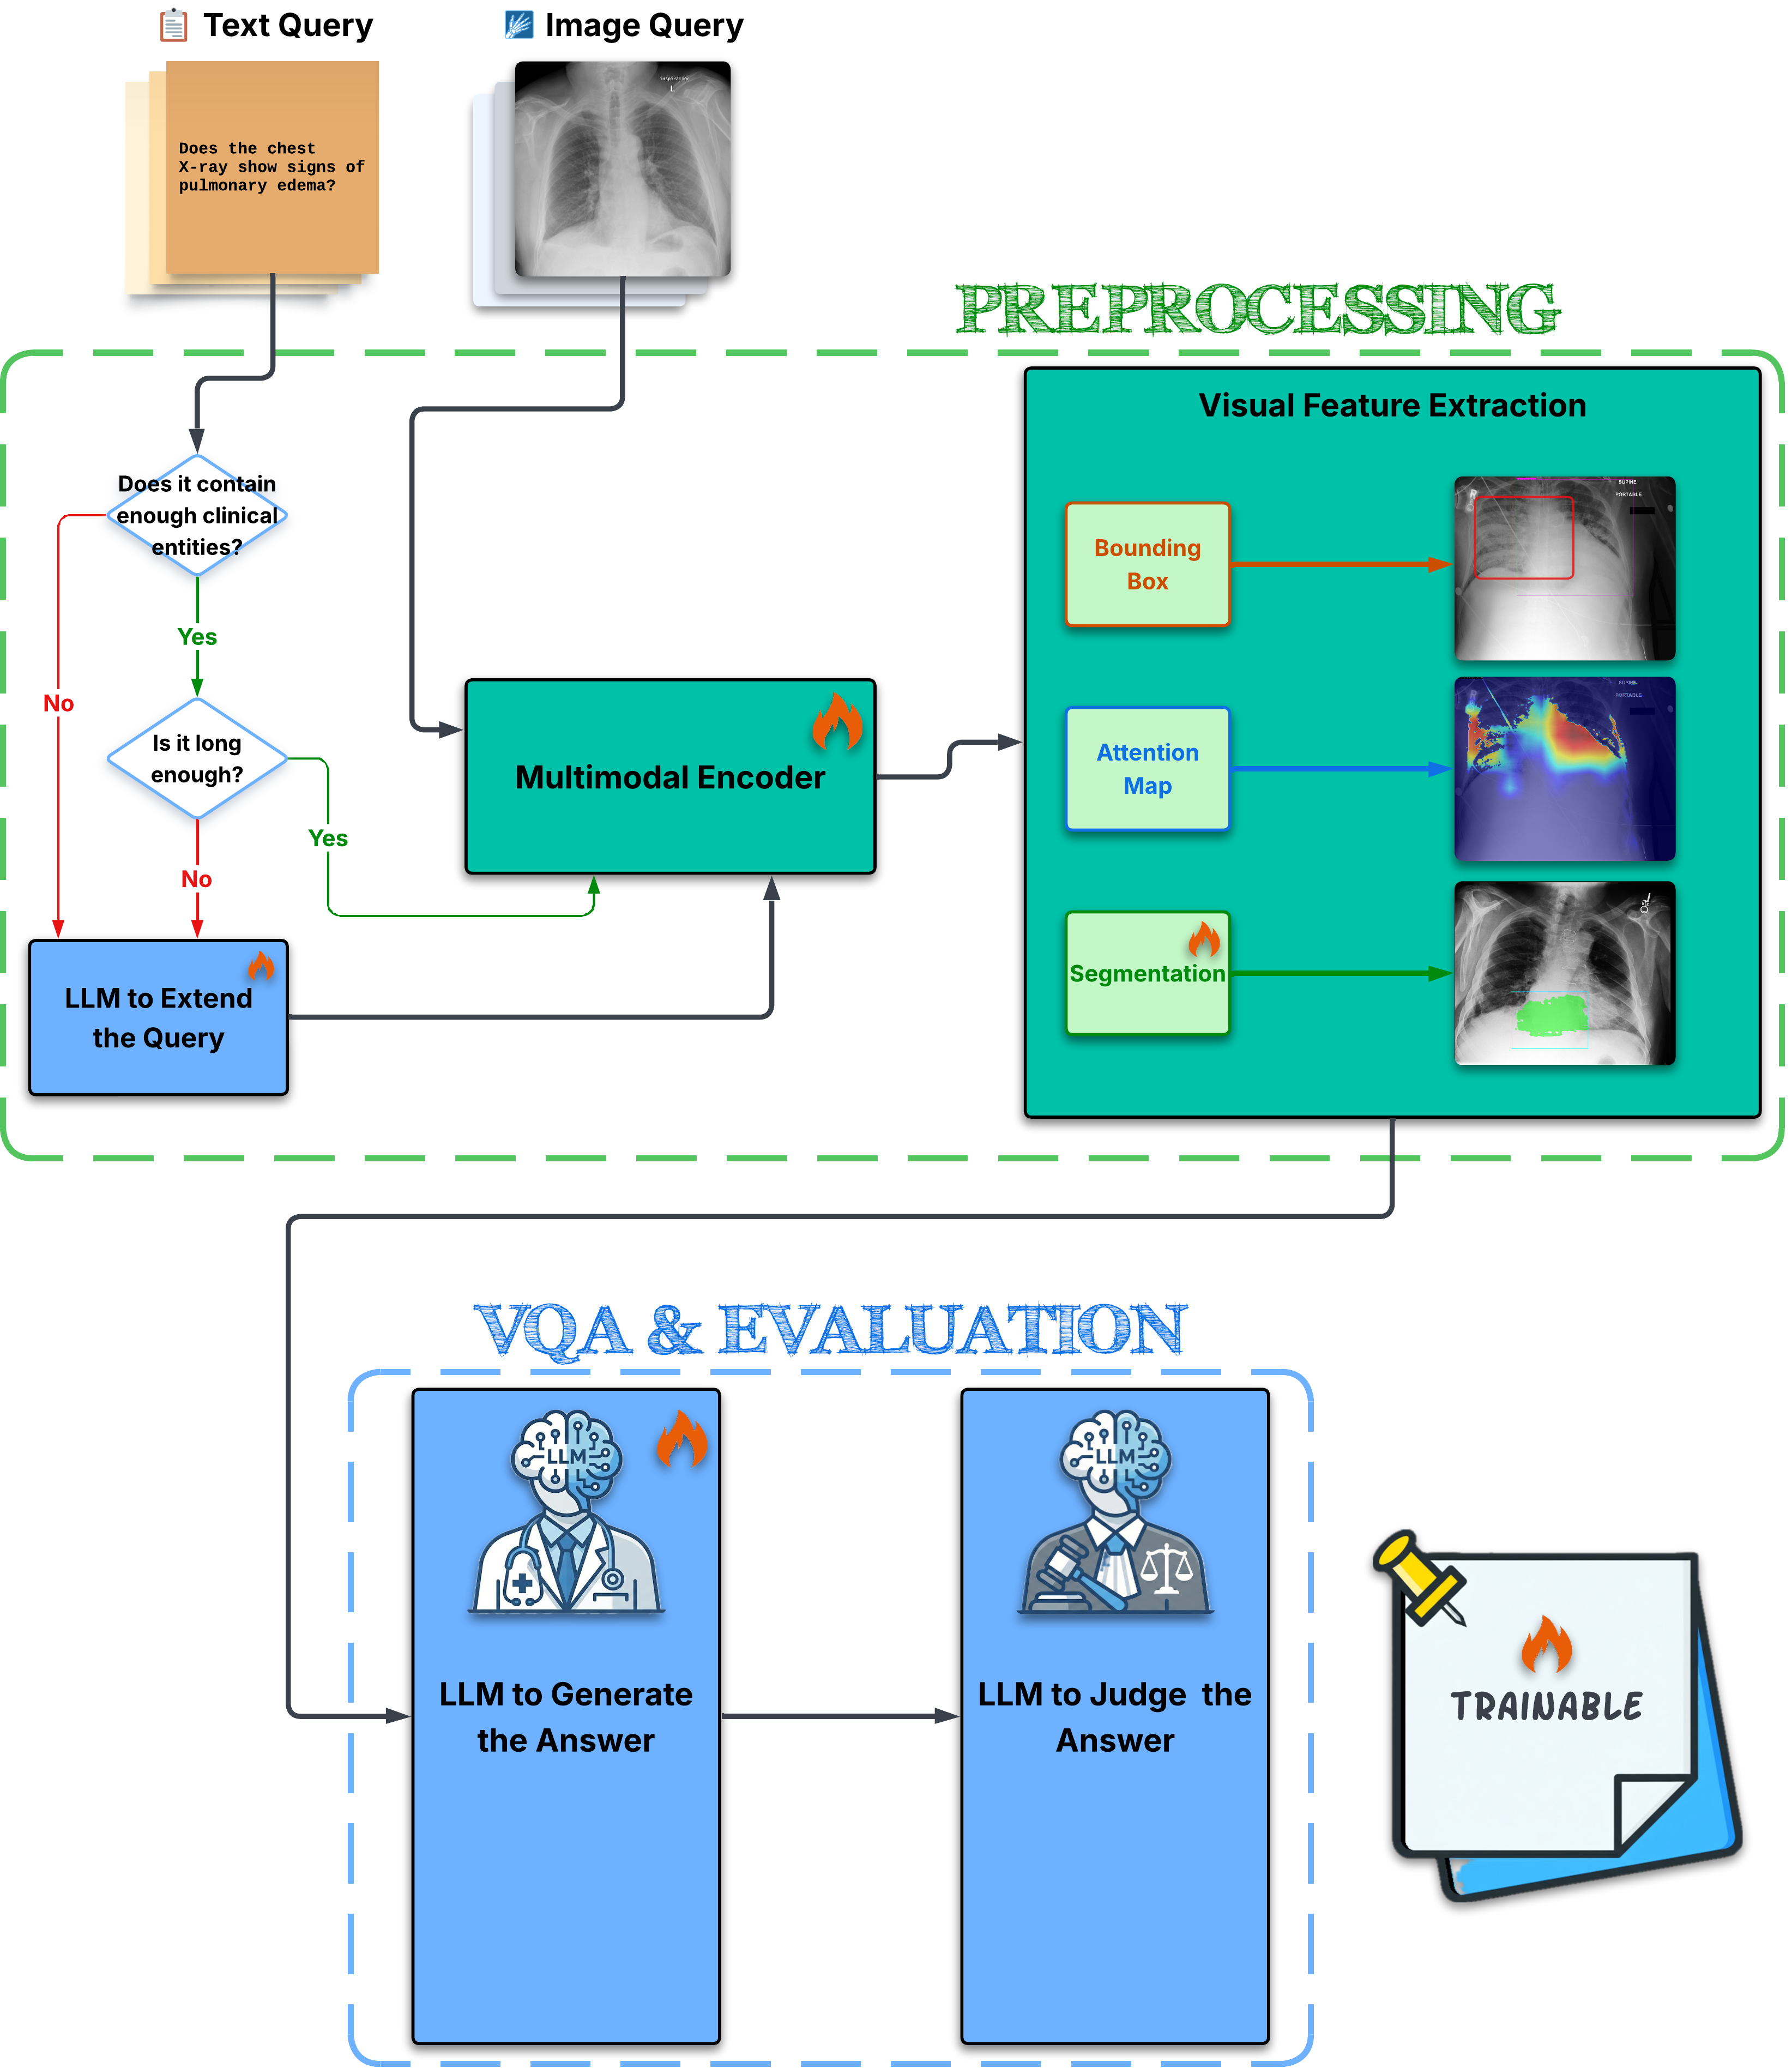
\includegraphics[width=1\linewidth]{real_pipeline.png}
    \caption{Enter Caption}
    \label{fig:placeholder}
\end{figure}

\section{Architectural Overview of the Pipeline}
\label{sec:3_1}
\subsection{Core Concept: Visual Grounding for Medical VQA}
\label{sec:3_1_1}

The central thesis underpinning the proposed system is that a Medical Visual Question Answering (VQA) model achieves superior diagnostic accuracy when it is not required to attend to an entire radiographic image indiscriminately, but is instead presented with a \textit{visually prompted} image in which the clinically relevant Regions of Interest (RoIs) have been explicitly highlighted. This paradigm, referred to throughout this work as \textbf{Visual Grounding}, transforms the VQA task from an unconstrained whole-image reasoning problem into a focused, region-aware inference problem.

Formally, let the raw input to the system be defined as a tuple $(\mathbf{I}, q)$, where $\mathbf{I} \in \mathbb{R}^{H \times W \times C}$ denotes a medical image (e.g., a chest X-ray) of height $H$, width $W$, and $C$ colour channels, and $q \in \mathcal{V}^*$ denotes a free-text clinical question drawn from the Kleene closure over a medical vocabulary $\mathcal{V}$. The objective of Visual Grounding is to construct an augmented image $\mathbf{I}' \in \mathbb{R}^{H \times W \times C}$ that encodes spatial emphasis on diagnostically salient regions, conditioned on the semantic content of $q$. The downstream VQA model $\mathcal{M}_{\text{VQA}}$ then operates on the pair $(\mathbf{I}', q)$ rather than $(\mathbf{I}, q)$, yielding a predicted answer:

\[
a^{*} = \mathcal{M}_{\text{VQA}}(\mathbf{I}', q)
\]

where:
\begin{itemize}
\item $a^{*}$ represents the predicted answer generated by the VQA model
\item $\mathcal{M}_{\text{VQA}}$ represents the downstream Vision-Language Model used for diagnostic answer generation
\item $\mathbf{I}' \in \mathbb{R}^{H \times W \times C}$ represents the visually prompted image encoding spatial emphasis on diagnostically salient regions
\item $q \in \mathcal{V}^*$ represents the free-text clinical question
\end{itemize}

The hypothesis is that the conditional mutual information between the answer $a^{*}$ and the ground-truth answer $a_{\text{gt}}$ is maximised when the visual input carries explicit spatial priors aligned with the clinical query—i.e., $I\left(a^{*}; a_{\text{gt}} \mid \mathbf{I}', q\right) \geq I\left(a^{*}; a_{\text{gt}} \mid I, q\right)$.

This design philosophy departs from end-to-end VQA architectures that implicitly learn visual attention. Instead, it externalises the grounding step as an explicit, interpretable preprocessing pipeline, thereby enabling clinical transparency, modular substitution of components, and fine-grained control over the spatial prompting strategy.

\subsection{End-to-End Data Flow}
\label{sec:3_1_2}
The pipeline implements a strictly sequential transformation chain comprising four macro-stages, each of which consumes the output of its predecessor. The complete data flow is formalised as:

\[
(\mathbf{I}, q) \xrightarrow{\;\mathcal{S}_1\;} q' \xrightarrow{\;\mathcal{S}_2\;} \mathbf{A} \xrightarrow{\;\mathcal{S}_3\;} \mathbf{I}' \xrightarrow{\;\mathcal{S}_4\;} a^{*}
\]

where the four stages are defined as follows:

\begin{itemize}
    \item \textbf{Stage $\mathcal{S}_1$ --- Clinical NLP Analysis (Query Routing).} The raw question $q$ is analysed by a biomedical Named Entity Recognition (NER) module $\mathcal{N}$ to assess its clinical informativeness. If the question is deemed insufficiently detailed according to a formally defined criterion (cf. \ref{sec:3_2}), it is expanded into an enriched clinical prompt $q'$ via a generative language model $\mathcal{G}$. If the question already satisfies the quality criterion, it is passed through unchanged, i.e., $q' = q$. This stage ensures that the downstream vision model receives a textual query of sufficient clinical specificity to drive meaningful spatial attention.

    \item \textbf{Stage $\mathcal{S}_2$ --- Visual Localisation via Cross-Modal Attention.} The enriched query $q'$ and the original image $\mathbf{I}$ are jointly encoded by a contrastive vision-language model $f_{\text{VL}}$---a dual-encoder architecture comprising a Vision Transformer (ViT) backbone and a domain-specific biomedical text encoder, pre-trained on large-scale biomedical image-text corpora---and a class activation mapping algorithm (gScoreCAM) is applied to produce a spatial attention map $\mathbf{A} \in \mathbb{R}^{H \times W}$, where each element $\mathbf{A}_{i,j} \in [0, 1]$ quantifies the relevance of pixel $(i, j)$ to the clinical query $q'$. This attention map constitutes the core localisation signal from which all subsequent visual prompts are derived.

    \item \textbf{Stage $\mathcal{S}_3$ --- Visual Prompting.} The attention map $\mathbf{A}$ is transformed into a concrete visual overlay on the original image $\mathbf{I}$. This stage admits multiple parallel pathways (detailed in Section \ref{sec:3_1_3}), each of which produces a differently prompted image $\mathbf{I}'$. The pathways share the same upstream attention signal but differ in their prompting semantics---ranging from geometric bounding boxes to dense pixel-level segmentation masks.

    \item \textbf{Stage $\mathcal{S}_4$ --- VQA Inference.} The visually prompted image $\mathbf{I}'$ is paired with the clinical question $q$ (or its expanded variant $q'$) and fed to a Vision-Language Model (VLM) for answer generation. A separate evaluation module employing an LLM-as-a-Judge paradigm scores the generated answer against the gold-standard reference.
\end{itemize}

The entire pipeline can thus be expressed as a composite function:

\[
\mathcal{F} = \mathcal{S}_4 \circ \mathcal{S}_3 \circ \mathcal{S}_2 \circ \mathcal{S}_1
\]

where each $\mathcal{S}_i$ is a deterministic, self-contained transformation with well-defined input and output types. This compositional structure guarantees that any individual stage can be replaced, ablated, or extended without affecting the contract between adjacent stages. %—a property that is exploited extensively in the experimental evaluation (Chapter 4).

\subsection{Modularity: Multiple Visual Prompting Pathways}
\label{sec:3_1_3}
A distinctive architectural decision in the proposed system is the provision of three distinct \textbf{Visual Prompting Pathways}, all of which branch from the same shared attention signal $\mathbf{A}$ produced by Stage $\mathcal{S}_2$. Each pathway implements a different strategy for converting the continuous-valued attention map into a discrete or semi-discrete visual prompt overlaid on the original image. This multi-pathway design serves a dual purpose: it enables systematic ablation studies comparing prompting strategies, and it accommodates the heterogeneous requirements of different downstream VLMs (some of which respond more effectively to bounding boxes than to heatmaps, and vice versa).

The three pathways are defined as follows:

\begin{itemize}

    \item \textbf{Pathway $\mathcal{P}_{\text{bbox}}$ --- Bounding Box Prompting.} The attention map $\mathbf{A}$ is binarised via a threshold $\tau$ (optionally refined through Dense CRF post-processing), and contour extraction is performed on the resulting binary mask. Each connected component yields a bounding box $\mathbf{b}_k = (x_k^{\min}, y_k^{\min}, x_k^{\max}, y_k^{\max})$, which is rendered as a coloured rectangle on the image. An adaptive padding mechanism adjusts the box margins as a function of the relative box area, preventing both excessive cropping of small findings and unnecessary expansion of large ones. The prompted image is:

    \[
    \mathbf{I}'_{\text{bbox}} = \text{DrawBox}(\mathbf{I}, \{\mathbf{b}_k\}_{k=1}^{K})
    \]

    where:
    \begin{itemize}
    \item $\mathbf{I}'_{\text{bbox}}$ represents the visually prompted image with bounding box overlays
    \item $\text{DrawBox}$ represents the rendering function that overlays coloured rectangles on the original image
    \item $\mathbf{I}$ represents the original medical image
    \item $\{\mathbf{b}_k\}_{k=1}^{K}$ represents the set of $K$ extracted bounding boxes, where each $\mathbf{b}_k = (x_k^{\min}, y_k^{\min}, x_k^{\max}, y_k^{\max})$
    \end{itemize}

    \item \textbf{Pathway $\mathcal{P}_{\text{heat}}$ --- Heatmap Overlay Prompting.} The raw attention map $\mathbf{A}$ is normalised to $[0, 1]$, mapped through a perceptual colourmap $\phi : [0,1] \to \mathbb{R}^3$ (e.g., JET or TURBO), and alpha-blended with the original image:

    \[
    \mathbf{I}'_{\text{heat}}(i,j) = \alpha \cdot \phi\!\left(\mathbf{A}_{i,j}\right) + (1 - \alpha) \cdot \mathbf{I}(i,j)
    \]

    where:
    \begin{itemize}
    \item $\mathbf{I}'_{\text{heat}}(i,j) \in \mathbb{R}^3$ represents the pixel value at coordinates $(i,j)$ of the heatmap-prompted image
    \item $\alpha \in [0, 1]$ represents the blending intensity coefficient controlling the opacity of the heatmap overlay
    \item $\phi : [0,1] \to \mathbb{R}^3$ represents the perceptual colourmap function mapping scalar attention values to RGB colour triples
    \item $\mathbf{A}_{i,j} \in [0,1]$ represents the normalised attention value at pixel $(i,j)$
    \item $\mathbf{I}(i,j) \in \mathbb{R}^C$ represents the original image pixel value at coordinates $(i,j)$
    \end{itemize}

    An optional anatomical body mask $\mathbf{M}_{\text{body}}$, computed via Otsu thresholding followed by morphological closing, suppresses attention activation in non-anatomical regions (e.g., textual annotations or imaging artefacts in the periphery of the radiograph).

    \item \textbf{Pathway $\mathcal{P}_{\text{seg}}$ --- Segmentation Mask Prompting.} The bounding boxes $\{\mathbf{b}_k\}$ extracted from $\mathbf{A}$ serve as geometric prompts for a dedicated segmentation foundation model $f_{\text{seg}}$, designed for medical image segmentation. The segmentation model produces a dense binary mask $\mathbf{M}_{\text{seg}} \in \{0, 1\}^{H \times W}$ that delineates the anatomical boundaries of the region of interest with pixel-level precision. The prompted image is generated by overlaying the mask contour or a semi-transparent filled mask onto the original image:

    \[
    \mathbf{I}'_{\text{seg}}(i,j) = \mathbf{M}_{\text{seg}}(i,j) \cdot \bigl[\beta \cdot c_{\text{mask}} + (1 - \beta) \cdot \mathbf{I}(i,j)\bigr] + \bigl(1 - \mathbf{M}_{\text{seg}}(i,j)\bigr) \cdot \mathbf{I}(i,j)
    \]

    where:
    \begin{itemize}
    \item $\mathbf{I}'_{\text{seg}}(i,j) \in \mathbb{R}^C$ represents the pixel value at coordinates $(i,j)$ of the segmentation-prompted image
    \item $\mathbf{M}_{\text{seg}}(i,j) \in \{0, 1\}$ represents the binary segmentation mask value at pixel $(i,j)$, where $1$ indicates foreground
    \item $\beta \in [0, 1]$ represents the mask opacity coefficient controlling the transparency of the segmentation overlay
    \item $c_{\text{mask}} \in \mathbb{R}^3$ represents the RGB overlay colour applied to segmented regions
    \item $\mathbf{I}(i,j) \in \mathbb{R}^C$ represents the original image pixel value at coordinates $(i,j)$
    \end{itemize}

    In the most advanced configuration, $f_{\text{seg}}$ accepts text prompts directly, enabling a complementary text-guided segmentation pathway that operates independently of the bounding box derivation.

\end{itemize}

All three pathways share the same upstream vision-language backbone $f_{\text{VL}}$ for attention computation, which ensures consistency of the localisation signal. The segmentation pathway additionally invokes a second, independent foundation model $f_{\text{seg}}$, creating a two-model cascade: the contrastive encoder $f_{\text{VL}}$ provides the \textit{where} (localisation), while the segmentation model $f_{\text{seg}}$ provides the \textit{what} (precise anatomical delineation). This cascaded architecture is summarised schematically below:

\[
\mathbf{A} = \text{gScoreCAM}\!\bigl(f_{\text{VL}}(\mathbf{I}, q')\bigr) \;\longrightarrow\; \begin{cases} \mathcal{P}_{\text{bbox}}(\mathbf{A}) \to \mathbf{I}'_{\text{bbox}} \\[4pt] \mathcal{P}_{\text{heat}}(\mathbf{A}) \to \mathbf{I}'_{\text{heat}} \\[4pt] \mathcal{P}_{\text{seg}}\!\bigl(f_{\text{seg}}(\mathbf{I}, \mathbf{b}(\mathbf{A}))\bigr) \to \mathbf{I}'_{\text{seg}} \end{cases}
\]

\subsection{Mathematical Abstraction of the Pipeline}
\label{sec:3_1_4}

To support rigorous experimental analysis, the complete pipeline is here abstracted as a parameterised composite function over well-typed intermediate representations.

Let $\mathcal{I} = \mathbb{R}^{H \times W \times C}$ denote the space of images, $\mathcal{Q} = \mathcal{V}^*$ the space of textual queries, and $\mathcal{A} = \mathcal{V}^*$ the space of natural-language answers. The four stages are typed as:

\[
\mathcal{S}_1 : \mathcal{Q} \to \mathcal{Q}' \quad \text{(Query Routing)}
\]

\[
\mathcal{S}_2 : \mathcal{I} \times \mathcal{Q}' \to [0, 1]^{H \times W} \quad \text{(Visual Localisation)}
\]

\[
\mathcal{S}_3^{(p)} : \mathcal{I} \times [0, 1]^{H \times W} \to \mathcal{I} \quad \text{(Visual Prompting, pathway } p \text{)}
\]

\[
\mathcal{S}_4 : \mathcal{I} \times \mathcal{Q}' \to \mathcal{A} \quad \text{(VQA Inference)}
\]

where $p \in \{\text{bbox}, \text{heat}, \text{seg}\}$ indexes the visual prompting pathway. The complete pipeline for a given pathway $p$ is then:

\[
\mathcal{F}^{(p)}(\mathbf{I}, q) = \mathcal{S}_4\!\Bigl(\mathcal{S}_3^{(p)}\!\bigl(\mathbf{I},\; \mathcal{S}_2(\mathbf{I},\; \mathcal{S}_1(q))\bigr),\; \mathcal{S}_1(q)\Bigr)
\]

This formulation makes explicit that the enriched query $q' = \mathcal{S}_1(q)$ is consumed by both the localisation stage $\mathcal{S}_2$ and the final VQA stage $\mathcal{S}_4$, establishing a dual information pathway: one visual (through $\mathcal{S}_2$ and $\mathcal{S}_3$) and one textual (direct bypass from $\mathcal{S}_1$ to $\mathcal{S}_4$). The attention map $\mathbf{A} = \mathcal{S}_2(\mathbf{I}, q')$ acts as a shared latent representation---a spatial ``bottleneck''---from which all visual prompting strategies diverge.

Each stage is governed by a set of hyperparameters $\theta_i$: for $\mathcal{S}_1$, these include the NER entity threshold and word-count threshold; for $\mathcal{S}_2$, the CAM variant, target layer index, and optional CRF parameters; for $\mathcal{S}_3^{(p)}$, the binarisation threshold $\tau$, blending coefficient $\alpha$, padding ratios, or segmentation model variant; and for $\mathcal{S}_4$, the choice of VLM and its generation hyperparameters. The full system is thus parameterised as:

\[
\mathcal{F}^{(p)}_{\Theta}(\mathbf{I}, q), \quad \Theta = (\theta_1, \theta_2, \theta_3^{(p)}, \theta_4)
\]

This parameterisation enables systematic grid-search experiments over the configuration space $\Theta$, the results of which are presented in Chapter 4.

\section{Clinical Text Preprocessing: Named Entity Recognition}
\label{sec:3_2}

\subsection{The Problem: Inadequacy of Raw Clinical Queries for Visual Grounding}
\label{sec:3_2_1}

The efficacy of the Visual Grounding pipeline described in Section \ref{sec:3_1} is fundamentally contingent upon the quality of the textual query $q$ that drives the cross-modal attention mechanism. The attention map
$\mathbf{A} = \text{gScoreCAM}(f_{\text{VL}}(\mathbf{I}, q))$ is, by construction, a function of both the image and the text: a vague or underspecified query will produce a diffuse, uninformative attention map that fails to localise any clinically meaningful region, regardless of the quality of the visual encoder.

In practice, clinical VQA datasets exhibit considerable heterogeneity in question quality. While some queries are highly specific and clinically rich (e.g., \textit{``Is there evidence of bilateral pleural effusion with associated compressive atelectasis in the lower lobes?''}), others are terse and ambiguous (e.g., \textit{``What is shown?''} or \textit{``Any findings?''}). The latter category poses a severe challenge for text-conditioned attention: the biomedical text encoder $f_{\text{text}}$, which maps $q$ to a fixed-dimensional embedding $\mathbf{t} = f_{\text{text}}(q) \in \mathbb{R}^d$, will project such underspecified queries into a region of the embedding space that is poorly discriminative with respect to spatial features, yielding near-uniform attention distributions that carry no localisation signal.

This problem is compounded by the domain specificity of medical language. General-purpose NLP models---including widely adopted NER systems trained predominantly on news corpora, web text, and general-domain encyclopaedic sources---fail to recognise clinical entities such as anatomical structures (e.g., \textit{costophrenic angle}, \textit{cardiomediastinal silhouette}), pathological findings (e.g., \textit{consolidation}, \textit{pneumothorax}), and imaging-specific terminology (e.g., \textit{opacification}, \textit{air bronchograms}). A general-purpose tokeniser may parse \textit{``bilateral pleural effusion''} as three independent tokens without recognising the phrase as a single clinical entity, thereby losing the compositional semantics that are critical for precise visual grounding.

The Clinical NLP Analysis stage ($\mathcal{S}_1$) is therefore designed to serve a dual function: (i) it \textit{evaluates} whether the raw query $q$ possesses sufficient clinical specificity to drive meaningful attention, and (ii) if the query is found deficient, it \textit{expands} it into a richer clinical prompt $q'$ via a generative language model $\mathcal{G}$. This section details the NER-based evaluation criterion that constitutes the first half of this mechanism.

\subsection{Methodology: Biomedical Named Entity Recognition}
\label{sec:3_2_2}
The evaluation of query quality is performed using a \textbf{Clinical Named Entity Recognition (NER)} module $\mathcal{N}$, built upon a specialised biomedical language pipeline trained on large-scale scientific corpora. Unlike general-purpose NER systems, this module leverages a domain-specific model whose tokeniser, part-of-speech tagger, dependency parser, and entity recogniser have been trained on a combination of biomedical corpora---including annotated biomedical abstracts and clinical text repositories---enabling the recognition of entities belonging to the Unified Medical Language System (UMLS) semantic categories.

The recognised entity categories encompass:

\begin{itemize}
    \item \textbf{Anatomical structures}: \textit{lung}, \textit{pleura}, \textit{mediastinum}, \textit{costophrenic angle}, \textit{trachea};
    \item \textbf{Pathological findings}: \textit{effusion}, \textit{consolidation}, \textit{pneumothorax}, \textit{cardiomegaly}, \textit{atelectasis};
    \item \textbf{Medical procedures and devices}: \textit{endotracheal tube}, \textit{central venous catheter}, \textit{sternotomy};
    \item \textbf{Clinical descriptors}: \textit{bilateral}, \textit{diffuse}, \textit{focal}, \textit{acute}, \textit{chronic}.
\end{itemize}

This domain-specific entity vocabulary is what distinguishes a biomedical NER module from general-purpose alternatives: where a standard general-domain NER model would fail to identify \textit{``pleural effusion''} as a meaningful entity, the biomedical NER module $\mathcal{N}$ correctly recognises it as a single clinical named entity, thereby preserving its compositional clinical semantics.

The NER extraction procedure is formalised as follows. Given a clinical query $q$, the biomedical NER module $\mathcal{N}$ processes the text and produces a document object from which a set of named entities is extracted:

$$
\mathcal{E}(q) = \{e_1, e_2, \ldots, e_n\} = \text{NER}_{\mathcal{N}}(q)
$$

where:
\begin{itemize}
\item $\mathcal{E}(q)$ represents the set of biomedical named entities extracted from query $q$
\item $e_i \in \mathcal{V}^+$ represents the $i$-th contiguous span of tokens recognised as a biomedical entity
\item $n = |\mathcal{E}(q)| \in \mathbb{N}_0$ represents the cardinality of the entity set, quantifying the clinical informativeness of the query
\item $\text{NER}_{\mathcal{N}}$ represents the Named Entity Recognition function parameterised by the biomedical NER module $\mathcal{N}$
\item $q$ represents the raw clinical query string
\end{itemize}

\subsection{Mathematical Framework: The Query Quality Decision Function}
\label{sec:3_2_3}
The decision as to whether a query $q$ requires expansion is governed by a binary decision function $\delta : \mathcal{Q} \to \{0, 1\}$ defined over two observable features: the number of detected clinical entities $n = |\mathcal{E}(q)|$ and the total word count $w = |q|_{\text{words}}$, computed as the number of whitespace-delimited tokens.

The decision function implements a conjunctive threshold criterion:

$$
\delta(q) = \begin{cases} 1 & \text{if } |\mathcal{E}(q)| \geq \tau_e \;\;\text{and}\;\; |q|_{\text{words}} \geq \tau_w \\ 0 & \text{otherwise} \end{cases}
$$

where:
\begin{itemize}
\item $\delta(q) \in \{0, 1\}$ represents the binary decision function output, with $1$ indicating a clinically detailed query and $0$ indicating a brief query requiring expansion
\item $|\mathcal{E}(q)| \in \mathbb{N}_0$ represents the number of biomedical named entities detected in query $q$
\item $|q|_{\text{words}} \in \mathbb{N}$ represents the total word count of query $q$, computed as the number of whitespace-delimited tokens
\item $\tau_e \in \mathbb{N}$ represents the \textbf{entity threshold} (default: $\tau_e = 2$), the minimum number of clinical entities required
\item $\tau_w \in \mathbb{N}$ represents the \textbf{word-count threshold} (default: $\tau_w = 5$), the minimum lexical extent required
\end{itemize}

A query $q$ is classified as \textit{clinically detailed} (and thus passed through unchanged) if and only if $\delta(q) = 1$. Conversely, a query for which $\delta(q) = 0$ is classified as \textit{brief} and is routed to the generative expansion module.

The conjunctive nature of this criterion is deliberate. The entity count condition alone would be insufficient, as a single-word medical term (e.g., \textit{``Pneumothorax?''}) may be parsed as one entity while still lacking the specificity required for grounded attention. Similarly, the word count condition alone would misclassify verbose but clinically vacuous queries (e.g., \textit{``Can you tell me what you see in this image?''}) as detailed. The conjunction of both conditions ensures that only queries possessing both sufficient lexical extent \textit{and} adequate clinical entity density are accepted without modification.

The routing logic is then expressed as:

$$
q' = \mathcal{S}_1(q) = \begin{cases} q & \text{if } \delta(q) = 1 \\ \text{Expand}(q; \mathcal{G}) & \text{if } \delta(q) = 0 \end{cases}
$$

where:
\begin{itemize}
\item $q' \in \mathcal{V}^*$ represents the enriched clinical prompt output by Stage $\mathcal{S}_1$
\item $\mathcal{S}_1$ represents the Clinical NLP Analysis stage (Query Routing)
\item $q$ represents the raw input clinical query
\item $\delta(q) \in \{0, 1\}$ represents the binary decision function defined above
\item $\text{Expand}(q; \mathcal{G})$ represents the output of the generative expansion module parameterised by the language model $\mathcal{G}$, which rewrites the brief query into a detailed clinical prompt of up to $L_{\max}$ new tokens, constrained to a single sentence by post-hoc truncation at the first newline character
\end{itemize}

\subsection{Implementation: NER Extraction and Conditional Routing}
\label{sec:3_2_4}

The implementation of the query quality evaluation and conditional routing logic is realised in two closely coupled functions. The first, \texttt{evaluate\_query\_quality}, encapsulates the NER extraction and the threshold-based decision:

\begin{pythoncode}[Query Quality Evaluation]
def evaluate_query_quality(
    nlp,
    query: str,
    entity_threshold: int = 2,
    word_threshold: int = 5,
) -> Tuple[bool, List[str]]:
    """
    Evaluate whether a text query is detailed enough for visual grounding.

    Heuristic:
    - The query must contain at least `entity_threshold` clinical entities.
    - The query must be at least `word_threshold` words long.
    """
    doc = nlp(query)
    entities = [ent.text for ent in doc.ents]
    word_count = len(query.split())

    is_detailed = (
        len(entities) >= entity_threshold and word_count >= word_threshold
    )
    return is_detailed, entities
\end{pythoncode}

The function accepts the preloaded biomedical NER model \texttt{nlp}, the raw query string, and the two configurable thresholds. The NER pipeline processes the query through its full NLP stack---tokenisation, POS tagging, dependency parsing, and NER---producing a document object from which entity spans are extracted as a list of surface-form strings. The word count is computed via whitespace tokenisation (\texttt{query.split()}), and the conjunctive threshold criterion $\delta(q)$ is evaluated. The function returns both the Boolean decision and the list of extracted entities, the latter being preserved in the output record for downstream traceability and analysis.

The second component is the conditional routing logic within the main processing loop, which orchestrates the interaction between the quality evaluation and the generative expansion:

\begin{pythoncode}[Conditional Routing Logic]
# --- Step 1: Query Quality Evaluation ---
is_detailed, entities = evaluate_query_quality(
    nlp, query,
    entity_threshold=args.entity_threshold,
    word_threshold=args.word_threshold,
)

# --- Step 2: Conditional Query Expansion ---
final_query = query
was_expanded = False
if not is_detailed:
    final_query = expand_query(
        gemma_model, gemma_tokenizer,
        query,
        max_new_tokens=args.gemma_max_new_tokens,
    )
    was_expanded = True
\end{pythoncode}

This excerpt illustrates the clean separation of concerns between the evaluation and expansion stages. The \texttt{evaluate\_query\_quality} function acts as a gatekeeper: only queries that fail the conjunctive threshold criterion are forwarded to the computationally more expensive generative language model $\mathcal{G}$, which requires GPU inference. The biomedical NER evaluation, by contrast, runs on CPU with negligible latency, yielding significant computational savings through conditional routing.

The output of Stage $\mathcal{S}_1$ is persisted as a structured record file in which each entry retains the original question, the (potentially expanded) query, the Boolean expansion flag, and the list of detected entities. This rich provenance information enables post-hoc analysis of the expansion rate and its correlation with downstream VQA performance.

\subsection{Bridging to Vision: From Clinical Entities to Spatial Attention Anchors}
\label{sec:3_2_5}

The clinical entities extracted by the NER module $\mathcal{N}$ in Stage $\mathcal{S}_1$ serve a purpose that extends beyond the immediate routing decision. They constitute the \textbf{textual anchors} that drive the cross-modal attention mechanism in Stage $\mathcal{S}_2$. To understand this bridging role, it is necessary to consider how the text encoder $f_{\text{text}}$ within $f_{\text{VL}}$ processes the enriched query $q'$.

The contrastive vision-language model $f_{\text{VL}}$ employs a domain-specific biomedical text encoder $f_{\text{text}}$ that maps the tokenised query into a $d$-dimensional embedding:

\[
\mathbf{t} = f_{\text{text}}(q') \in \mathbb{R}^d
\]

where:
\begin{itemize}
\item $\mathbf{t} \in \mathbb{R}^d$ represents the continuous textual embedding vector
\item $f_{\text{text}}$ represents the domain-specific biomedical textual encoder function
\item $q'$ represents the enriched clinical prompt (output of Stage $\mathcal{S}_1$)
\item $d$ represents the dimensionality of the shared latent embedding space
\end{itemize}

This embedding is then compared against the spatial feature map produced by the ViT visual encoder $f_{\text{vis}}$. In the gScoreCAM algorithm, the activation of the target layer---specifically, the output of the final normalisation sublayer in the last transformer block---yields a spatial feature tensor $\mathbf{F} \in \mathbb{R}^{N \times d}$, where $N = (H/P) \times (W/P)$ is the number of spatial tokens in the ViT grid for patch size $P$. The attention score for spatial position $j$ is computed as a function of the similarity between $\mathbf{t}$ and the channel-masked perturbations of $\mathbf{F}$, producing the final attention map:

\[
\mathbf{A}_{j} = \text{gScoreCAM}(\mathbf{F}, \mathbf{t})_j, \quad j \in \{1, \ldots, N\}
\]

where:
\begin{itemize}
\item $\mathbf{A}_{j} \in [0,1]$ represents the attention score at spatial position $j$ in the ViT grid
\item $\text{gScoreCAM}$ represents the grouped Score-weighted Class Activation Mapping algorithm
\item $\mathbf{F} \in \mathbb{R}^{N \times d}$ represents the spatial feature tensor from the target ViT layer
\item $\mathbf{t} \in \mathbb{R}^d$ represents the textual embedding of the enriched query $q'$
\item $N = (H/P) \times (W/P)$ represents the number of spatial tokens in the ViT grid for patch size $P$
\end{itemize}

The clinical entities in $q'$ directly influence the text embedding $\mathbf{t}$ and, consequently, the spatial distribution of attention. A query enriched with specific anatomical entities (e.g., \textit{``pleural effusion''}, \textit{``costophrenic angle''}) will produce a text embedding that is highly discriminative in the joint embedding space of $f_{\text{VL}}$, activating spatial tokens that correspond to the relevant anatomical structures. Conversely, a vague query that has not undergone expansion will produce a text embedding in a poorly localised region of the joint space, resulting in diffuse or noisy attention.

This establishes the critical link between the NLP preprocessing of Section \ref{sec:3_2} and the visual localisation of Section \ref{sec:3_3} (to follow): the quality of the attention map $\mathbf{A}$---and, by extension, the precision of all downstream visual prompts---is a direct function of the clinical specificity of the entities embedded in $q'$. The biomedical NER module $\mathcal{N}$ therefore acts not merely as a text filter, but as a \textbf{quality assurance mechanism} for the entire visual grounding pipeline, ensuring that the textual signal driving cross-modal attention is of sufficient clinical granularity to produce spatially meaningful localisation.

\section{Attention Map Generation: Contrastive Vision-Language Encoder and gScoreCAM}
\label{sec:3_3}
\subsection{The Contrastive Vision-Language Backbone}
\label{sec:3_3_1}

\subsubsection{Architecture and Pretraining}
\label{sec:3_3_1_1}

The vision-language backbone $f_{\text{VL}}$ employed throughout the pipeline is a \textbf{contrastive vision-language encoder} pre-trained on a large-scale biomedical image-text corpus comprising millions of figure-caption pairs from the biomedical literature. The model follows a CLIP-style dual-encoder architecture in which a visual encoder $f_{\text{vis}}$ and a textual encoder $f_{\text{text}}$ are jointly trained to maximise cosine similarity between matched image-text pairs while minimising it for unmatched pairs, thereby learning a shared, semantically aligned latent space.

\textbf{Visual Encoder $f_{\text{vis}}$: Vision Transformer (ViT).} An input image $\mathbf{I} \in \mathbb{R}^{H_0 \times W_0 \times 3}$ is partitioned into non-overlapping $P \times P$ patches, yielding $N = (H_0/P) \times (W_0/P)$ patch tokens.  Each patch is linearly projected into $\mathbb{R}^d$, a learnable CLS token $\mathbf{z}_{\text{CLS}}$ is prepended, and positional embeddings are added, producing a sequence of $N + 1$ tokens. This sequence is processed through $L$ transformer blocks in a pre-norm configuration:

$$
\mathbf{Z}^{(\ell)} = \text{FFN}\!\bigl(\text{LN}(\mathbf{H}^{(\ell)})\bigr) + \mathbf{H}^{(\ell)}, \quad \mathbf{H}^{(\ell)} = \text{MHSA}\!\bigl(\text{LN}(\mathbf{Z}^{(\ell-1)})\bigr) + \mathbf{Z}^{(\ell-1)}
$$

where:
\begin{itemize}
\item $\mathbf{Z}^{(\ell)}$ represents the output token sequence of transformer block $\ell$
\item $\mathbf{H}^{(\ell)}$ represents the intermediate representation after the multi-head self-attention sub-layer in block $\ell$
\item $\text{MHSA}$ represents the Multi-Head Self-Attention operation
\item $\text{FFN}$ represents the position-wise Feed-Forward Network
\item $\text{LN}$ represents Layer Normalisation (pre-norm configuration)
\item $\mathbf{Z}^{(\ell-1)}$ represents the input token sequence from the preceding block
\end{itemize}

for $\ell = 1, \ldots, L$. The final image embedding is:

$$
\mathbf{v} = \text{Proj}_{\text{vis}}\!\bigl(\mathbf{Z}^{(L)}_{\text{CLS}}\bigr) \in \mathbb{R}^d
$$

where:
\begin{itemize}
\item $\mathbf{v} \in \mathbb{R}^d$ represents the final continuous visual embedding vector
\item $\text{Proj}_{\text{vis}}$ represents the visual projection head mapping the CLS token to the shared embedding space
\item $\mathbf{Z}^{(L)}_{\text{CLS}}$ represents the CLS token output from the final ($L$-th) transformer block
\item $d$ represents the dimensionality of the shared latent embedding space
\end{itemize}

\textbf{Textual Encoder $f_{\text{text}}$: Domain-Specific Biomedical Encoder.} A biomedical language model pre-trained on scientific abstracts receives the tokenised query $q'$ and produces a text embedding via [CLS] pooling:

$$
\mathbf{t} = f_{\text{text}}(q') \in \mathbb{R}^d
$$

where:
\begin{itemize}
\item $\mathbf{t} \in \mathbb{R}^d$ represents the continuous textual embedding vector obtained via [CLS] pooling
\item $f_{\text{text}}$ represents the domain-specific biomedical textual encoder function
\item $q'$ represents the enriched clinical query
\end{itemize}

The text encoder's vocabulary and representations are specifically tuned on biomedical text, enabling high-fidelity encoding of the clinical entities produced by the NER module $\mathcal{N}$ of Section \ref{sec:3_2}.

\subsubsection{Cross-Modal Similarity Computation}
\label{sec:3_3_1_2}

The two encoders are united through a contrastive similarity objective. Given $\ell_2$-normalised embeddings, the model computes their dot-product similarity scaled by a learned temperature $\lambda$:

$$
s(\mathbf{I}, q') = \lambda \cdot \hat{\mathbf{v}}^{\top} \hat{\mathbf{t}}, \quad \hat{\mathbf{v}} = \frac{\mathbf{v}}{\|\mathbf{v}\|_2}, \quad \hat{\mathbf{t}} = \frac{\mathbf{t}}{\|\mathbf{t}\|_2}
$$

where:
\begin{itemize}
\item $s(\mathbf{I}, q') \in \mathbb{R}$ represents the scaled cross-modal similarity score between the image $\mathbf{I}$ and the query $q'$
\item $\lambda = \exp(\text{logit\_scale}) \in \mathbb{R}_{>0}$ represents the learned temperature parameter that sharpens discrimination between matched and unmatched pairs
\item $\hat{\mathbf{v}}, \hat{\mathbf{t}} \in \mathbb{R}^d$ represent the $\ell_2$-normalised visual and textual embeddings, respectively
\item $\mathbf{v}, \mathbf{t} \in \mathbb{R}^d$ represent the raw visual and textual embedding vectors prior to normalisation
\end{itemize} A critical design decision is the \textbf{decoupling of text encoding from the visual forward pass}: the text embedding $\hat{\mathbf{t}}$ is pre-computed and cached before CAM computation. During ScoreCAM perturbation (Section \ref{sec:3_3_2}), the visual encoder is executed multiple times while the text embedding remains fixed---semantically correct (the query is invariant across perturbations) and computationally efficient (the text encoder is invoked only once). This wrapper class encapsulates the computation:

\begin{pythoncode}[BiomedCLIPWrapper]
class BiomedCLIPWrapper(nn.Module):
    def __init__(self, model: nn.Module):
        super().__init__()
        self.model = model
        self.text_embeddings = None

    def set_text(self, text_tokens: torch.Tensor):
        with torch.no_grad():
            emb = self.model.encode_text(text_tokens)
            self.text_embeddings = emb / emb.norm(dim=-1, keepdim=True)

    def forward(self, images: torch.Tensor, texts=None) -> torch.Tensor:
        image_embeddings = self.model.encode_image(images)
        image_embeddings = image_embeddings / image_embeddings.norm(
            dim=-1, keepdim=True
        )
        logit_scale = self.model.logit_scale.exp()
        logits = logit_scale * image_embeddings @ self.text_embeddings.t()
        return logits
\end{pythoncode}

The output is a similarity logit matrix $\mathbf{S} \in \mathbb{R}^{B_I \times B_T}$. In single-prompt mode, $B_T = 1$ and $\mathbf{S}$ is a column vector. In composite multi-region mode, $B_T = B_I = N$ and each diagonal element $\mathbf{S}_{i,i}$ encodes the similarity between image $i$ and its corresponding prompt $i$.

\subsection{The gScoreCAM Algorithm}
\label{sec:3_3_2}

\subsubsection{Motivation: Gradient-Free Attribution for Vision Transformers}
\label{sec:3_3_2_1}

Classical Grad-CAM computes the gradient of the target score with respect to a convolutional layer's activation maps, using these gradients as importance weights. While effective for CNNs, this approach is problematic for Vision Transformers: the global self-attention mechanism breaks the locality assumption underpinning Grad-CAM, and gradients in deep transformers suffer from saturation and noise propagation, yielding diffuse, unreliable saliency maps.

 \textbf{ScoreCAM} (and its grouped variant, \textbf{gScoreCAM}) eliminates gradient dependency entirely via a \textbf{perturbation-based} strategy: each channel of the target layer's activation is used as a spatial mask on the input, and the resulting change in the model's output score is measured directly through forward passes. This is inherently more stable for ViTs, as it evaluates the functional impact of each feature channel without relying on backpropagated gradients.

\subsubsection{Mathematical Formulation}

Let $\mathbf{F}^{(\ell)} \in \mathbb{R}^{D \times h \times w}$ denote the activation tensor at target layer $\ell$, where $D$ is the channel dimension and $h \times w$ is the spatial resolution after the reshape transform. For each channel $k \in \{1, \ldots, D\}$, the spatial activation slice $\mathbf{F}_k^{(\ell)} \in \mathbb{R}^{h \times w}$ is min-max normalised:

\[
\hat{\mathbf{F}}_k = \frac{\mathbf{F}_k^{(\ell)} - \min(\mathbf{F}_k^{(\ell)})}{\max(\mathbf{F}_k^{(\ell)}) - \min(\mathbf{F}_k^{(\ell)}) + \epsilon}
\]

where:
\begin{itemize}
\item $\hat{\mathbf{F}}_k \in [0,1]^{h \times w}$ represents the min-max normalised spatial activation for channel $k$
\item $\mathbf{F}_k^{(\ell)} \in \mathbb{R}^{h \times w}$ represents the raw spatial activation slice at channel $k$ of target layer $\ell$
\item $\epsilon > 0$ is a small constant for numerical stability
\end{itemize}

The normalised activation is upsampled to input resolution and used as a soft spatial mask:

\[
\mathbf{I}_k^{\text{masked}} = \hat{\mathbf{F}}_k^{\uparrow} \odot \mathbf{I}
\]

where:
\begin{itemize}
\item $\mathbf{I}_k^{\text{masked}}$ represents the spatially masked input image obtained by modulating $\mathbf{I}$ with the $k$-th channel activation
\item $\hat{\mathbf{F}}_k^{\uparrow} \in [0,1]^{H \times W}$ represents the normalised activation of channel $k$, upsampled to input resolution
\item $\odot$ denotes element-wise (Hadamard) multiplication, broadcast across colour channels
\item $\mathbf{I}$ represents the original input image
\end{itemize}

The weight $w_k$ is defined as the \textbf{increase in confidence} induced by the masked image relative to a baseline:

\[
w_k = s\!\left(\mathbf{I}_k^{\text{masked}}, q'\right) - s\!\left(\mathbf{I}_{\text{baseline}}, q'\right)
\]

where:
\begin{itemize}
\item $w_k \in \mathbb{R}$ represents the importance weight for channel $k$, measuring the increase in cross-modal similarity induced by the masked image
\item $s(\cdot, q')$ represents the scaled similarity function between an image and the enriched query $q'$
\item $\mathbf{I}_k^{\text{masked}}$ represents the input image modulated by the $k$-th channel activation
\item $\mathbf{I}_{\text{baseline}}$ represents the baseline image (typically a zero or blurred input)
\end{itemize}

The final attention map is a ReLU-gated weighted sum of all normalised activations:

\[
\mathbf{A} = \text{ReLU}\!\left(\sum_{k=1}^{D} w_k \cdot \hat{\mathbf{F}}_k^{\uparrow}\right)
\]

where:
\begin{itemize}
\item $\mathbf{A} \in [0,1]^{H \times W}$ represents the final attention map (spatial saliency signal)
\item $\text{ReLU}$ represents the Rectified Linear Unit, suppressing negative activations
\item $D$ represents the total number of channels in the target layer
\item $w_k \in \mathbb{R}$ represents the perturbation-derived importance weight for channel $k$
\item $\hat{\mathbf{F}}_k^{\uparrow} \in [0,1]^{H \times W}$ represents the normalised and upsampled activation of channel $k$
\end{itemize}

\subsubsection{Grouped ScoreCAM (gScoreCAM): Computational Efficiency}

Standard ScoreCAM requires $D$ forward passes---one per channel. For large $D$, this is computationally expensive. \textbf{gScoreCAM} reduces this cost by selecting the top-$G$ channels ranked by spatial activation variance. Channels with low variance carry no localisation signal and are discarded:

\[
\mathbf{A} = \text{ReLU}\!\left(\sum_{k \in \mathcal{T}_G} w_k \cdot \hat{\mathbf{F}}_k^{\uparrow}\right), \quad |\mathcal{T}_G| = \min(G, D)
\]

where:
\begin{itemize}
\item $\mathcal{T}_G \subseteq \{1, \ldots, D\}$ represents the subset of top-$G$ channels ranked by spatial activation variance
\item $G$ represents the number of retained channels (a configurable hyperparameter)
\item $D$ represents the total number of channels in the target layer
\end{itemize}

\subsection{Target Layer Selection and Feature Extraction}

 The target layer for gScoreCAM is set to the \textbf{second layer normalisation} of the final transformer block in $f_{\text{vis}}$:

\begin{pythoncode}[Target Layer Selection]
target_layer = self.clip_model.model.visual.trunk.blocks[11].norm2
\end{pythoncode}

The final block encodes the richest semantic-spatial representations, as $L$ successive self-attention layers have aggregated both local texture and global context. Within this block, the second normalisation sublayer---applied after the FFN---captures the complete transformed representation:

\[
\mathbf{Z}^{(L)}_{\text{norm2}} = \text{LN}\!\left(\text{FFN}\!\bigl(\text{LN}(\mathbf{H}^{(L)})\bigr) + \mathbf{H}^{(L)}\right)
\]

where:
\begin{itemize}
\item $\mathbf{Z}^{(L)}_{\text{norm2}}$ represents the output of the second layer normalisation in the final ($L$-th) transformer block
\item $\text{LN}$ represents Layer Normalisation
\item $\text{FFN}$ represents the position-wise Feed-Forward Network
\item $\mathbf{H}^{(L)}$ represents the intermediate representation after the multi-head self-attention sub-layer in block $L$
\end{itemize}

This tensor of shape $(B, N+1, D)$ is reshaped into a spatial activation tensor $\mathbf{F}^{(\ell)} \in \mathbb{R}^{B \times D \times h \times w}$ by the \texttt{reshape\_transform} function: the CLS token is removed, the $N$ remaining tokens are arranged into an $h \times w$ grid ($h = w = \sqrt{N}$), and the tensor is permuted to $(B, D, h, w)$:

\begin{pythoncode}[Reshape Transform Function]
def reshape_transform(tensor, height=None, width=None):
    patches = tensor[:, 1:, :]  # Remove CLS token
    num_patches = patches.shape[1]
    grid_side = int(num_patches ** 0.5)
    height = width = grid_side
    result = patches.reshape(
        tensor.shape[0], height, width, tensor.shape[2]
    )
    result = result.permute(0, 3, 1, 2)  # (B, D, H, W)
    return result
\end{pythoncode}

Each position in the $h \times w$ grid has a nominal $P \times P$ receptive field but an effective receptive field spanning the entire image due to global self-attention, enabling the encoder to attend to anatomically distributed findings from any single spatial token.

\subsection{Pipeline Initialisation and Batch Inference}

The inference pipeline class encapsulates model loading, tokeniser configuration, target layer selection, and CAM wrapper instantiation:

\begin{pythoncode}[BiomedCLIPInferencePipeline]
class BiomedCLIPInferencePipeline:
    def __init__(self, args, device='cuda'):
        self.device = device
        self.cam_version = args.cam_version  # Default: 'gScoreCAM'

        _, _, _, self.cam_transform, _ = load_clip(args.clip_version)
        biomed_core, self.preprocess = open_clip.create_model_from_pretrained(
            args.model_name  # 'hf-hub:microsoft/BiomedCLIP-...'
        )
        self.tokenizer = SafeBiomedTokenizer(args.model_name)
        biomed_core.to(self.device).eval()
        self.clip_model = BiomedCLIPWrapper(biomed_core)

        target_layer = self.clip_model.model.visual.trunk.blocks[11].norm2
        self.cam_wrapper = BatchCAMWrapper(
            model=self.clip_model,
            target_layers=[target_layer],
            tokenizer=self.tokenizer,
            cam_version=self.cam_version,
            topk=args.topk,
            is_transformer=True,
            cam_trans=self.cam_transform
        )
\end{pythoncode}

Batch inference is handled by a dedicated method that distinguishes two cases. In \textbf{Case A} (uniform prompts), a single text embedding is cached and the entire batch is processed simultaneously. In \textbf{Case B} (composite multi-region mode), each image is paired with a distinct anatomical prompt. All $N$ text embeddings are computed in one batched call, producing the similarity matrix:

$$
\mathbf{S} = \lambda \cdot \hat{\mathbf{V}} \, \hat{\mathbf{T}}^{\top}
$$

where:
\begin{itemize}
\item $\mathbf{S} \in \mathbb{R}^{N \times N}$ represents the similarity logit matrix, where each entry $\mathbf{S}_{i,j}$ encodes the scaled similarity between image $i$ and prompt $j$
\item $\lambda \in \mathbb{R}_{>0}$ represents the learned temperature parameter
\item $\hat{\mathbf{V}} \in \mathbb{R}^{N \times d}$ represents the matrix of $\ell_2$-normalised visual embeddings for all $N$ images in the batch
\item $\hat{\mathbf{T}} \in \mathbb{R}^{N \times d}$ represents the matrix of $\ell_2$-normalised textual embeddings for all $N$ prompts
\end{itemize}

A target selection mechanism ensures that the CAM for the $i$-th image targets the diagonal element $\mathbf{S}_{i,i}$, correctly attributing each region-specific attention map to its paired prompt.

\subsection{Post-Processing: Normalisation, Masking, and CRF Refinement}

The raw attention map $\mathbf{A}_{\text{raw}}$ on the ViT grid must be post-processed before consumption by the downstream visual prompting pathways (Section \ref{sec:3_1_3}) or binarisation for bounding box extraction (Section \ref{sec:3_4}).

\subsubsection{Anatomical Body Masking}


Radiographic images frequently contain non-anatomical artefacts (patient identification text, laterality markers, collimation borders) that can produce spurious attention activations. An optional \textbf{anatomical body mask} $\mathbf{M}_{\text{body}} \in \{0, 1\}^{H \times W}$ is computed in three stages:

\textbf{Stage A --- Body Detection.} Otsu's method automatically determines a binarisation threshold maximising between-class variance:

$$
\tau^{*} = \arg\max_{\tau} \, \sigma^2_B(\tau)
$$

where:
\begin{itemize}
\item $\tau^{*}$ represents the optimal binarisation threshold determined automatically by Otsu's method
\item $\sigma^2_B(\tau) \in \mathbb{R}_{\geq 0}$ represents the between-class variance at threshold $\tau$, quantifying the separability of the foreground and background intensity distributions
\end{itemize}

The mask is refined via morphological closing to fill intrabody holes, followed by dilation for a conservative margin.

\textbf{Stage B --- White Artefact Detection.} Pixels exceeding a high-intensity threshold are identified as digital text or markers and dilated to cover anti-aliased edges, producing a glare mask $\mathbf{M}_{\text{glare}}$.

\textbf{Stage C --- Fusion.} The final mask is the set difference:

$$
\mathbf{M}_{\text{body}} = \mathbf{M}_{\text{Otsu}} \setminus \mathbf{M}_{\text{glare}}
$$

where:
\begin{itemize}
\item $\mathbf{M}_{\text{body}} \in \{0,1\}^{H \times W}$ represents the final anatomical body mask
\item $\mathbf{M}_{\text{Otsu}} \in \{0,1\}^{H \times W}$ represents the body region mask obtained via Otsu thresholding and morphological refinement
\item $\mathbf{M}_{\text{glare}} \in \{0,1\}^{H \times W}$ represents the white artefact mask identifying high-intensity non-anatomical pixels
\item $\setminus$ denotes the set difference operator, retaining only body pixels that are not artefacts
\end{itemize}

The mask is resized to CAM resolution via nearest-neighbour interpolation and applied element-wise:

$$
\mathbf{A}_{\text{masked}} = \mathbf{A}_{\text{raw}} \odot \mathbf{M}_{\text{body}}^{\downarrow}
$$

where:
\begin{itemize}
\item $\mathbf{A}_{\text{masked}}$ represents the attention map after anatomical masking
\item $\mathbf{A}_{\text{raw}}$ represents the raw attention map on the ViT spatial grid
\item $\mathbf{M}_{\text{body}}^{\downarrow}$ represents the anatomical body mask downsampled to CAM resolution via nearest-neighbour interpolation
\item $\odot$ denotes element-wise (Hadamard) multiplication
\end{itemize}

\subsubsection{Min-Max Normalisation}

The masked map is normalised to $[0, 1]$:

$$
\mathbf{A}_{\text{norm}}(i,j) = \frac{\mathbf{A}_{\text{masked}}(i,j) - \min(\mathbf{A}_{\text{masked}})}{\max(\mathbf{A}_{\text{masked}}) - \min(\mathbf{A}_{\text{masked}}) + \epsilon}
$$

where:
\begin{itemize}
\item $\mathbf{A}_{\text{norm}}(i,j) \in [0,1]$ represents the normalised attention value at pixel $(i,j)$
\item $\mathbf{A}_{\text{masked}}(i,j)$ represents the masked attention value at pixel $(i,j)$
\item $\min(\mathbf{A}_{\text{masked}}), \max(\mathbf{A}_{\text{masked}})$ represent the global minimum and maximum values over the entire masked attention map
\item $\epsilon > 0$ is a small constant ensuring numerical stability
\end{itemize}

If $\max - \min \leq \epsilon$, the map is zeroed (no localisation signal detected). The normalised map is then bilinearly upsampled to the original resolution:

$$
\mathbf{A} = \text{Resize}(\mathbf{A}_{\text{norm}}, H, W)
$$

where:
\begin{itemize}
\item $\mathbf{A} \in [0,1]^{H \times W}$ represents the final attention map upsampled to the original image resolution
\item $\text{Resize}$ represents the bilinear interpolation upsampling function
\item $\mathbf{A}_{\text{norm}}$ represents the normalised attention map at CAM resolution
\item $H, W$ represent the height and width of the original input image
\end{itemize}

This $\mathbf{A} \in [0, 1]^{H \times W}$ is the canonical output of Stage $\mathcal{S}_2$: for the heatmap pathway ($\mathcal{P}_{\text{heat}}$), it is directly colourmap-rendered and alpha-blended; for the bounding box ($\mathcal{P}_{\text{bbox}}$) and segmentation ($\mathcal{P}_{\text{seg}}$) pathways, it undergoes binarisation as described in Section \ref{sec:3_4}.

\subsubsection{Dense CRF Refinement (Optional)}


For the bounding box pathway, fixed-threshold binarisation of $\mathbf{A}$ often produces fragmented boundaries, particularly for diffuse findings. An optional \textbf{Dense CRF} post-processing step refines the map before binarisation.

The CRF operates on a two-class formulation with unary potentials derived from the attention map:

$$
U_{\text{fg}}(i,j) = -\log\!\bigl(\mathbf{A}_{\text{norm}}(i,j) + \epsilon\bigr), \quad U_{\text{bg}}(i,j) = -\log\!\bigl(1 - \mathbf{A}_{\text{norm}}(i,j) + \epsilon\bigr)
$$

where:
\begin{itemize}
\item $U_{\text{fg}}(i,j) \in \mathbb{R}_{\geq 0}$ represents the unary potential (cost) for assigning pixel $(i,j)$ to the foreground class
\item $U_{\text{bg}}(i,j) \in \mathbb{R}_{\geq 0}$ represents the unary potential (cost) for assigning pixel $(i,j)$ to the background class
\item $\mathbf{A}_{\text{norm}}(i,j) \in [0,1]$ represents the normalised attention value at pixel $(i,j)$, serving as a foreground likelihood prior
\item $\epsilon > 0$ is a small constant ensuring numerical stability of the logarithm
\end{itemize}

Pairwise potentials enforce spatial smoothness via two kernels. A \textbf{Gaussian kernel} penalises label disagreements between proximate pixels:

$$
\psi_{\text{G}}(\mathbf{p}, \mathbf{p}') = \mu_{\text{G}} \cdot \exp\!\left(-\frac{\|\mathbf{p} - \mathbf{p}'\|^2}{2\sigma_{\text{xy}}^2}\right)
$$

where:
\begin{itemize}
\item $\psi_{\text{G}}(\mathbf{p}, \mathbf{p}') \in \mathbb{R}_{\geq 0}$ represents the smoothness penalty between pixels at positions $\mathbf{p}$ and $\mathbf{p}'$
\item $\mu_{\text{G}} \in \mathbb{R}_{>0}$ represents the weight of the Gaussian smoothness kernel
\item $\mathbf{p}, \mathbf{p}' \in \mathbb{R}^2$ represent the spatial coordinates of two pixels
\item $\sigma_{\text{xy}} \in \mathbb{R}_{>0}$ represents the spatial bandwidth controlling the range of influence
\end{itemize}

A \textbf{bilateral kernel} additionally conditions on image appearance:

$$
\psi_{\text{B}}(\mathbf{p}, \mathbf{p}') = \mu_{\text{B}} \cdot \exp\!\left(-\frac{\|\mathbf{p} - \mathbf{p}'\|^2}{2\sigma_{\text{xy}}^{\text{bil}\,2}} - \frac{\|\mathbf{I}(\mathbf{p}) - \mathbf{I}(\mathbf{p}')\|^2}{2\sigma_{\text{rgb}}^2}\right)
$$

where:
\begin{itemize}
\item $\psi_{\text{B}}(\mathbf{p}, \mathbf{p}') \in \mathbb{R}_{\geq 0}$ represents the appearance-sensitive bilateral penalty between pixels at positions $\mathbf{p}$ and $\mathbf{p}'$
\item $\mu_{\text{B}} \in \mathbb{R}_{>0}$ represents the weight of the bilateral kernel
\item $\sigma_{\text{xy}}^{\text{bil}} \in \mathbb{R}_{>0}$ represents the spatial bandwidth of the bilateral kernel
\item $\sigma_{\text{rgb}} \in \mathbb{R}_{>0}$ represents the chromatic bandwidth controlling sensitivity to intensity differences
\item $\mathbf{I}(\mathbf{p}), \mathbf{I}(\mathbf{p}')$ represent the pixel intensity values in the original image at positions $\mathbf{p}$ and $\mathbf{p}'$
\end{itemize}

Mean-field inference is performed for $M$ iterations, yielding a refined foreground probability map for contour extraction and bounding box generation in Section \ref{sec:3_4}.

%%%%%%%%%%%%%%%%%%%%%%%%%%%%%%%%%%%%%%%%%%%%%%
% CAPITOLO 3 (da 3.4 a 3.5)                  %
%%%%%%%%%%%%%%%%%%%%%%%%%%%%%%%%%%%%%%%%%%%%%%

\section{Advanced Bounding Box Extraction}
\label{sec:3_4}

The continuous attention map $\mathbf{A} \in [0,1]^{H \times W}$ produced by Stage $\mathcal{S}_2$ (Section~\ref{sec:3_3}) encodes a soft, pixel-level estimate of clinical relevance conditioned on the textual query $q'$. However, the bounding box prompting pathway $\mathcal{P}_{\text{bbox}}$ and the segmentation prompting pathway $\mathcal{P}_{\text{seg}}$ both require discrete geometric primitives---specifically, axis-aligned bounding rectangles $\mathbf{b}_k = (x_k^{\min}, y_k^{\min}, x_k^{\max}, y_k^{\max})$---as input. The transformation from a continuous saliency signal to a set of tight, semantically coherent bounding boxes is therefore a critical and mathematically non-trivial step.

Na\"ive fixed-threshold binarisation of $\mathbf{A}$ is insufficient in practice: the attention map may exhibit heterogeneous intensity distributions across different images and clinical queries, and a single global threshold cannot adapt to this variability. Furthermore, raw binarised masks frequently suffer from:

\begin{itemize}
  \item ~\textit{salt-and-pepper noise} in low-activation regions, producing spurious small components;
  \item ~\textit{fragmented boundaries} around diffuse findings such as pleural effusions, where attention gradients are smooth rather than sharp;
  \item ~\textit{over-merging} of distinct but adjacent findings into a single connected component
\end{itemize}


This section presents the mathematical framework underlying the three post-processing techniques that address these challenges: adaptive thresholding via Otsu's method (Section~\ref{sec:3_4_1}), morphological enhancement via the Top-Hat transform (Section~\ref{sec:3_4_2}), and boundary refinement via Dense Conditional Random Fields (Section~\ref{sec:3_4_3}). Together, these operations constitute the core of Stage $\mathcal{S}_3^{(\text{bbox})}$: the conversion of the shared attention signal $\mathbf{A}$ into the discrete set of bounding boxes $\{\mathbf{b}_k\}_{k=1}^{K}$ that define the Regions of Interest.

\subsection{Image Binarisation via Otsu's Method}
\label{sec:3_4_1}

The first step in extracting bounding boxes from the continuous attention map $\mathbf{A}$ is the conversion of the grayscale saliency signal into a binary foreground-background mask. This requires the selection of a threshold $\tau^{*}$ that separates high-attention pixels (foreground, corresponding to clinically relevant regions) from low-attention pixels (background). Rather than relying on a fixed, manually tuned threshold---which would require per-dataset or per-query calibration---the pipeline employs \textbf{Otsu's method}, an automatic, histogram-based thresholding algorithm that determines the optimal threshold by minimising intra-class variance.

\subsubsection{Mathematical Formulation}

Let $\mathbf{A}$ be quantised to $L$ discrete intensity levels (typically $L = 256$ after scaling to the $[0, 255]$ range). The normalised histogram of $\mathbf{A}$ defines a probability distribution over intensity levels:

\begin{equation}
p_i = \frac{n_i}{N}, \quad i \in \{0, 1, \ldots, L-1\}
\end{equation}

where:
\begin{itemize}
\item $p_i \in [0,1]$ represents the probability that a pixel in the attention map assumes intensity level $i$
\item $n_i \in \mathbb{N}_0$ represents the count of pixels with intensity level $i$
\item $N = H \times W$ represents the total number of pixels in the attention map
\item $L \in \mathbb{N}$ represents the number of discrete intensity levels
\end{itemize}

A candidate threshold $\tau \in \{0, 1, \ldots, L-1\}$ partitions the pixel population into two classes: the background class $C_0 = \{i : i \leq \tau\}$ and the foreground class $C_1 = \{i : i > \tau\}$. For each class, the cumulative probability (class prior) and the conditional mean intensity are defined as:

\begin{equation}
\omega_0(\tau) = \sum_{i=0}^{\tau} p_i, \qquad \omega_1(\tau) = \sum_{i=\tau+1}^{L-1} p_i = 1 - \omega_0(\tau)
\end{equation}

\begin{equation}
\mu_0(\tau) = \frac{1}{\omega_0(\tau)} \sum_{i=0}^{\tau} i \cdot p_i, \qquad \mu_1(\tau) = \frac{1}{\omega_1(\tau)} \sum_{i=\tau+1}^{L-1} i \cdot p_i
\end{equation}

where:
\begin{itemize}
\item $\omega_0(\tau), \omega_1(\tau) \in [0,1]$ represent the class prior probabilities (cumulative pixel fractions) for the background and foreground classes, respectively
\item $\mu_0(\tau), \mu_1(\tau) \in \mathbb{R}$ represent the conditional mean intensity values of the background and foreground classes, respectively
\item $\tau$ represents the candidate threshold value partitioning the intensity histogram
\end{itemize}

The global mean intensity is $\mu_T = \omega_0(\tau)\,\mu_0(\tau) + \omega_1(\tau)\,\mu_1(\tau)$. Otsu's criterion selects the threshold that \textit{maximises the between-class variance} $\sigma_B^2(\tau)$, which is mathematically equivalent to minimising the weighted sum of intra-class variances:

\begin{equation}
\label{eq:otsu}
\tau^{*} = \arg\max_{\tau \in \{0, \ldots, L-1\}} \; \sigma_B^2(\tau) = \arg\max_{\tau} \; \omega_0(\tau)\,\omega_1(\tau)\,\bigl(\mu_0(\tau) - \mu_1(\tau)\bigr)^2
\end{equation}

where:
\begin{itemize}
\item $\tau^{*} \in \{0, \ldots, L-1\}$ represents the optimal threshold that maximises the separability between background and foreground intensity distributions
\item $\sigma_B^2(\tau) \in \mathbb{R}_{\geq 0}$ represents the between-class variance at threshold $\tau$, quantifying the separation between the two class means
\item $\omega_0(\tau), \omega_1(\tau)$ represent the class prior probabilities as defined above
\item $\mu_0(\tau), \mu_1(\tau)$ represent the conditional class means as defined above
\end{itemize}

The optimality of Equation~\ref{eq:otsu} follows from the total variance decomposition theorem: the total intensity variance $\sigma_T^2$ decomposes into $\sigma_T^2 = \sigma_W^2(\tau) + \sigma_B^2(\tau)$, where $\sigma_W^2$ is the weighted intra-class variance. Since $\sigma_T^2$ is constant with respect to $\tau$, maximising $\sigma_B^2$ is equivalent to minimising $\sigma_W^2$, ensuring the tightest possible separation between the two pixel populations.

\subsubsection{Application to the Attention Map}

Given the optimal threshold $\tau^{*}$ determined by Otsu's method, the binary mask $\mathbf{B} \in \{0, 1\}^{H \times W}$ is obtained via:

\begin{equation}
\mathbf{B}(i,j) = \begin{cases} 1 & \text{if } \mathbf{A}(i,j) > \tau^{*} / (L-1) \\ 0 & \text{otherwise} \end{cases}
\end{equation}

where:
\begin{itemize}
\item $\mathbf{B}(i,j) \in \{0,1\}$ represents the binary label (foreground or background) assigned to pixel $(i,j)$
\item $\mathbf{A}(i,j) \in [0,1]$ represents the normalised attention value at pixel $(i,j)$
\item $\tau^{*}/(L-1)$ represents the optimal threshold rescaled to the $[0,1]$ range of the normalised attention map
\end{itemize}

This automatic thresholding eliminates the need for per-image threshold tuning and naturally adapts to the attention intensity distribution of each specific image-query pair. For images where the attention map exhibits a clear bimodal histogram (i.e., well-separated foreground and background distributions), Otsu's method yields a sharp, high-quality binary separation. In cases where the attention distribution is unimodal or heavily skewed, the threshold tends toward conservative foreground selection, which is the preferred behaviour in a clinical setting where false negatives (missed findings) carry higher risk than over-segmented boxes.


\subsection{Morphological Enhancements: The Top-Hat Transform}
\label{sec:3_4_2}

The binary mask $\mathbf{B}$ obtained via Otsu's thresholding may still contain artefacts that degrade the quality of the extracted bounding boxes: isolated noise pixels in the background, thin bridges connecting otherwise distinct regions, and attenuated local peaks that fall below the global threshold. Classical morphological operators provide a principled mathematical framework for addressing these issues without altering the semantic content of the mask.

\subsubsection{Morphological Preliminaries}

Let $\mathbf{X} \subseteq \mathbb{Z}^2$ denote the set of foreground pixels and $\mathbf{S} \subseteq \mathbb{Z}^2$ a compact \textit{structuring element} (e.g., a disc or square of radius $r$). The two fundamental morphological operations are \textbf{erosion} and \textbf{dilation}:

\begin{equation}
\mathbf{X} \ominus \mathbf{S} = \{ \mathbf{z} \in \mathbb{Z}^2 : \mathbf{S}_{\mathbf{z}} \subseteq \mathbf{X} \}
\end{equation}

\begin{equation}
\mathbf{X} \oplus \mathbf{S} = \{ \mathbf{z} \in \mathbb{Z}^2 : \hat{\mathbf{S}}_{\mathbf{z}} \cap \mathbf{X} \neq \emptyset \}
\end{equation}

where:
\begin{itemize}
\item $\mathbf{X} \ominus \mathbf{S}$ denotes the erosion of $\mathbf{X}$ by $\mathbf{S}$, retaining only pixels whose translated structuring element is entirely contained within $\mathbf{X}$
\item $\mathbf{X} \oplus \mathbf{S}$ denotes the dilation of $\mathbf{X}$ by $\mathbf{S}$, expanding $\mathbf{X}$ to include all pixels that overlap with the translated reflected structuring element
\item $\mathbf{S}_{\mathbf{z}}$ represents the structuring element $\mathbf{S}$ translated to be centred at position $\mathbf{z}$
\item $\hat{\mathbf{S}}_{\mathbf{z}}$ represents the reflected structuring element translated to position $\mathbf{z}$
\end{itemize}

From these primitives, two composite operations are derived. The \textbf{morphological opening} $\mathbf{X} \circ \mathbf{S} = (\mathbf{X} \ominus \mathbf{S}) \oplus \mathbf{S}$ removes small protrusions and isolated noise components that are smaller than the structuring element, while globally preserving the shape and area of larger structures. The \textbf{morphological closing} $\mathbf{X} \bullet \mathbf{S} = (\mathbf{X} \oplus \mathbf{S}) \ominus \mathbf{S}$ fills small holes and narrow gaps within the foreground.

\subsubsection{The White Top-Hat Transform}

The \textbf{White Top-Hat transform} (also known simply as the Top-Hat transform) is defined as the residual between the original image and its morphological opening. When applied to the grayscale attention map $\mathbf{A}$ (rather than the binary mask), it isolates \textit{bright local features} whose spatial extent is smaller than the structuring element:

\begin{equation}
\label{eq:tophat}
\mathbf{T}_{\text{WTH}}(i,j) = \mathbf{A}(i,j) - (\mathbf{A} \circ \mathbf{S})(i,j)
\end{equation}

where:
\begin{itemize}
\item $\mathbf{T}_{\text{WTH}}(i,j) \in \mathbb{R}_{\geq 0}$ represents the White Top-Hat response at pixel $(i,j)$, quantifying the local brightness excess relative to the morphological background
\item $\mathbf{A}(i,j) \in [0,1]$ represents the original continuous attention value at pixel $(i,j)$
\item $(\mathbf{A} \circ \mathbf{S})(i,j)$ represents the morphological opening of $\mathbf{A}$ by structuring element $\mathbf{S}$, which estimates the local background intensity
\item $\mathbf{S}$ represents the structuring element, whose size governs the spatial scale of features to be extracted
\end{itemize}

The morphological opening $\mathbf{A} \circ \mathbf{S}$ acts as a non-linear low-pass filter: it suppresses features brighter than the local background that are smaller than $\mathbf{S}$, producing a smooth estimate of the background intensity surface. Subtracting this estimate from the original signal isolates precisely those local peaks and ridges that correspond to focal attention activations---the regions most likely to encode clinically salient findings.

\subsubsection{Application in the Pipeline}

In the bounding box extraction pipeline, the Top-Hat transform serves two complementary purposes:

\begin{enumerate}
    \item \textbf{Noise suppression:} By adjusting the size of the structuring element $\mathbf{S}$, activations whose spatial footprint falls below a clinically meaningful scale are removed. For a structuring element of radius $r$ pixels, only attention peaks spanning an area larger than approximately $\pi r^2$ pixels survive the transform. This effectively eliminates salt-and-pepper artefacts without requiring explicit connected-component filtering.

    \item \textbf{Peak enhancement:} Focal findings that produce sharp, localised attention peaks (e.g., small nodules or focal consolidations) are enhanced relative to the diffuse background, improving their visibility in the subsequent binarisation step. This is particularly beneficial when the Otsu threshold would otherwise subsume small but diagnostically significant activations into the background class.
\end{enumerate}

The enhanced attention map $\mathbf{A}_{\text{enh}} = \mathbf{A} + \gamma \cdot \mathbf{T}_{\text{WTH}}$, where $\gamma \in \mathbb{R}_{>0}$ is a weighting coefficient, is optionally substituted for $\mathbf{A}$ before Otsu thresholding. The parameter $\gamma$ and the structuring element size $r$ are included in the hyperparameter set $\theta_3^{(\text{bbox})}$ and are subject to grid-search optimisation (\ref{chap:4}).


\subsection{Boundary Refinement with Dense Conditional Random Fields}
\label{sec:3_4_3}

The binarised attention mask obtained via Otsu's thresholding---with or without morphological enhancement---produces boundaries that are globally consistent but locally imprecise. This is an inherent consequence of the attention map's spatial resolution: the gScoreCAM saliency signal originates from the spatial grid of the Vision Transformer, and even after bilinear upsampling to the full image resolution $H \times W$, the boundaries remain smooth and grid-aligned rather than conforming to the true anatomical contours present in the original image. \textbf{Dense Conditional Random Fields (CRFs)} address this limitation by incorporating the pixel-level appearance information of the original image $\mathbf{I}$ into the labelling process.

\subsubsection{Probabilistic Formulation}

A Dense CRF models the joint probability of a pixel-wise label assignment $\mathbf{x} = \{x_1, x_2, \ldots, x_N\}$ over all $N = H \times W$ pixels, where each $x_i \in \{0, 1\}$ denotes the background or foreground label for pixel $i$. The CRF defines a Gibbs distribution:

\begin{equation}
P(\mathbf{x} \mid \mathbf{I}, \mathbf{A}) = \frac{1}{Z} \exp\!\bigl(-E(\mathbf{x})\bigr)
\end{equation}

where:
\begin{itemize}
\item $P(\mathbf{x} \mid \mathbf{I}, \mathbf{A}) \in [0,1]$ represents the conditional probability of the label configuration $\mathbf{x}$ given the input image $\mathbf{I}$ and the attention map $\mathbf{A}$
\item $Z = \sum_{\mathbf{x}'} \exp(-E(\mathbf{x}'))$ represents the partition function ensuring normalisation over all possible label configurations
\item $E(\mathbf{x}) \in \mathbb{R}$ represents the Gibbs energy function of the configuration $\mathbf{x}$
\end{itemize}

The maximum a posteriori (MAP) labelling $\mathbf{x}^{*} = \arg\min_{\mathbf{x}} E(\mathbf{x})$ yields the optimal foreground-background segmentation. The energy function decomposes into unary and pairwise terms:

\begin{equation}
\label{eq:crf_energy}
E(\mathbf{x}) = \sum_{i=1}^{N} \psi_u(x_i) + \sum_{i < j} \psi_p(x_i, x_j)
\end{equation}

where:
\begin{itemize}
\item $\psi_u(x_i) \in \mathbb{R}_{\geq 0}$ represents the unary potential for pixel $i$, encoding the cost of assigning label $x_i$ based on the attention map evidence
\item $\psi_p(x_i, x_j) \in \mathbb{R}_{\geq 0}$ represents the pairwise potential between pixels $i$ and $j$, encoding the cost of assigning different labels to spatially or chromatically proximate pixels
\end{itemize}

\subsubsection{Unary Potentials}

The unary potentials are derived directly from the normalised attention map $\mathbf{A}_{\text{norm}}$, which provides a per-pixel estimate of foreground membership likelihood. For each pixel $i$ with spatial coordinates $(i_x, i_y)$:

\begin{equation}
\psi_u(x_i = 1) = -\log\!\bigl(\mathbf{A}_{\text{norm}}(i_x, i_y) + \epsilon\bigr)
\end{equation}

\begin{equation}
\psi_u(x_i = 0) = -\log\!\bigl(1 - \mathbf{A}_{\text{norm}}(i_x, i_y) + \epsilon\bigr)
\end{equation}

where:
\begin{itemize}
\item $\psi_u(x_i = 1), \psi_u(x_i = 0) \in \mathbb{R}_{\geq 0}$ represent the unary costs of assigning pixel $i$ to the foreground and background classes, respectively
\item $\mathbf{A}_{\text{norm}}(i_x, i_y) \in [0,1]$ represents the normalised attention value at the spatial coordinates of pixel $i$, serving as a soft foreground prior
\item $\epsilon > 0$ is a small constant ensuring numerical stability of the logarithm
\end{itemize}

This formulation ensures that pixels with high attention values incur low foreground cost and high background cost, and vice versa. The negative logarithm converts the attention-derived probabilities into additive energy terms consistent with the Gibbs framework.

\subsubsection{Pairwise Potentials}

The pairwise potentials encode the spatial and chromatic compatibility between pixel pairs, encouraging label smoothness while respecting image boundaries. Following the formulation of fully connected (dense) CRFs, the pairwise potential between pixels $i$ and $j$ is defined as a weighted mixture of Gaussian kernels applied to feature vectors:

\begin{equation}
\label{eq:crf_pairwise}
\begin{aligned}
\psi_p(x_i, x_j) = \mu(x_i, x_j) \biggl[ & \mu_{\text{G}} \cdot \exp\left(-\frac{\|\mathbf{p}_i - \mathbf{p}_j\|^2}{2\sigma_{\text{xy}}^2}\right) \\
& + \mu_{\text{B}} \cdot \exp\left(-\frac{\|\mathbf{p}_i - \mathbf{p}_j\|^2}{2\sigma_{\text{xy}}^{\text{bil}\,2}} - \frac{\|\mathbf{I}_i - \mathbf{I}_j\|^2}{2\sigma_{\text{rgb}}^2}\right) \biggr]
\end{aligned}
\end{equation}

where:
\begin{itemize}
\item $\mu(x_i, x_j) = \mathbb{1}[x_i \neq x_j]$ is the Potts compatibility function, equal to $1$ when pixels $i$ and $j$ carry different labels and $0$ otherwise, ensuring that the pairwise penalty is applied only to label disagreements
\item $\mathbf{p}_i, \mathbf{p}_j \in \mathbb{R}^2$ represent the spatial coordinates of pixels $i$ and $j$
\item $\mathbf{I}_i, \mathbf{I}_j \in \mathbb{R}^C$ represent the colour (or intensity) vectors of pixels $i$ and $j$ in the original image $\mathbf{I}$
\item $\mu_{\text{G}} \in \mathbb{R}_{>0}$ represents the weight of the \textit{smoothness kernel}, which penalises label disagreements between spatially proximate pixels regardless of their appearance
\item $\mu_{\text{B}} \in \mathbb{R}_{>0}$ represents the weight of the \textit{appearance kernel} (bilateral kernel), which additionally conditions the penalty on chromatic similarity
\item $\sigma_{\text{xy}} \in \mathbb{R}_{>0}$ represents the spatial bandwidth of the smoothness kernel, controlling the range of spatial influence
\item $\sigma_{\text{xy}}^{\text{bil}} \in \mathbb{R}_{>0}$ represents the spatial bandwidth of the bilateral kernel
\item $\sigma_{\text{rgb}} \in \mathbb{R}_{>0}$ represents the chromatic bandwidth of the bilateral kernel, controlling sensitivity to colour differences
\end{itemize}

The two kernels fulfil complementary roles. The \textbf{smoothness kernel} (first term) enforces spatial coherence by penalising label transitions between nearby pixels, thereby suppressing isolated noise pixels and producing contiguous foreground regions. The \textbf{appearance kernel} (second term) preserves true boundaries: when two pixels are close in space but differ significantly in intensity (as occurs at anatomical boundaries in radiographic images), the bilateral term attenuates the smoothness penalty, permitting the label assignment to respect the image gradient.

\subsubsection{Mean-Field Inference}

Exact MAP inference in a fully connected CRF is computationally intractable due to the $\mathcal{O}(N^2)$ pairwise interactions. The efficient mean-field approximation factorises the posterior into independent marginals $Q(\mathbf{x}) = \prod_{i} Q_i(x_i)$ and iteratively updates each marginal via message passing. Each iteration involves three steps: (1)~computing the pairwise messages as Gaussian-filtered marginal distributions, (2)~weighting by compatibility, and (3)~updating the marginals by combining unary potentials with incoming messages. This is performed for $M$ iterations (typically $M = 5$--$10$), after which the refined foreground probability map $Q_i(x_i = 1)$ replaces the raw attention-derived labelling.

The resulting refined mask preserves the global structure of the attention-based binarisation while aligning the boundaries to the intensity gradients of the original radiographic image. This is particularly beneficial for diffuse pathologies (e.g., pleural effusions, ground-glass opacities) where the attention signal provides correct coarse localisation but the precise extent of the finding is best determined by the underlying image contrast.

\subsection{Contour Extraction and Bounding Box Derivation}
\label{sec:3_4_4}

The final step in the bounding box extraction pipeline operates on the refined binary mask---obtained either directly from Otsu thresholding, after morphological enhancement, or after CRF refinement. Connected component analysis identifies the set of maximal connected foreground regions $\{R_k\}_{k=1}^{K}$. For each connected component $R_k$, the minimum enclosing axis-aligned bounding box is computed:

\begin{equation}
\mathbf{b}_k = \bigl(\min_{(i,j) \in R_k} j, \;\; \min_{(i,j) \in R_k} i, \;\; \max_{(i,j) \in R_k} j, \;\; \max_{(i,j) \in R_k} i\bigr)
\end{equation}

where:
\begin{itemize}
\item $\mathbf{b}_k = (x_k^{\min}, y_k^{\min}, x_k^{\max}, y_k^{\max}) \in \mathbb{N}^4$ represents the bounding box coordinates for the $k$-th connected component
\item $R_k \subseteq \{1,\ldots,H\} \times \{1,\ldots,W\}$ represents the set of pixel coordinates belonging to the $k$-th connected foreground region
\item $K \in \mathbb{N}$ represents the total number of detected connected components (i.e., distinct Regions of Interest)
\end{itemize}

An \textbf{adaptive padding} mechanism subsequently expands each bounding box by a margin proportional to the relative box area, defined as $\rho_k = |\mathbf{b}_k| / (H \times W)$, where $|\mathbf{b}_k|$ denotes the area of the box. Small boxes (high clinical specificity, small $\rho_k$) receive proportionally larger margins to capture the surrounding anatomical context, while large boxes (low specificity, large $\rho_k$) receive minimal expansion to avoid encompassing irrelevant regions. The padding ratio is governed by a piecewise-linear function parameterised by thresholds in $\theta_3^{(\text{bbox})}$.

The final set of padded bounding boxes $\{\mathbf{b}_k\}_{k=1}^{K}$ is rendered as coloured rectangles on the original image $\mathbf{I}$, producing the visually prompted image:

\[
\mathbf{I}'_{\text{bbox}} = \text{DrawBox}\!\bigl(\mathbf{I}, \{\mathbf{b}_k\}_{k=1}^{K}\bigr)
\]

This image serves as input to either the downstream VQA model $\mathcal{M}_{\text{VQA}}$ (in the bounding box pathway) or as geometric prompts for the segmentation foundation model $f_{\text{seg}}$ (in the segmentation pathway $\mathcal{P}_{\text{seg}}$).

%----------------------------------------------

\section{From Mathematical Framework to System Realisation}
\label{sec:3_5}

\subsection{Synthesis of the Proposed Methodology}

The preceding sections have established a complete, mathematically grounded framework for Visual Grounding in Medical VQA. The methodology proceeds through a rigorously defined transformation chain:

\begin{enumerate}
    \item \textbf{Clinical Text Preprocessing} (Section~\ref{sec:3_2}): A biomedical NER module $\mathcal{N}$ evaluates the clinical informativeness of the raw query $q$ through a conjunctive threshold criterion $\delta(q)$ over entity count and lexical extent. Queries that fail this criterion are expanded via a generative language model $\mathcal{G}$, producing an enriched clinical prompt $q'$ that provides sufficient semantic specificity to drive cross-modal attention.

    \item \textbf{Attention Map Generation} (Section~\ref{sec:3_3}): The enriched query $q'$ and the medical image $\mathbf{I}$ are jointly processed by the contrastive vision-language backbone $f_{\text{VL}}$, and a gradient-free class activation mapping algorithm (gScoreCAM) extracts a continuous attention map $\mathbf{A} \in [0,1]^{H \times W}$ that quantifies the spatial relevance of each pixel to the clinical query.

    \item \textbf{Bounding Box Extraction} (Section~\ref{sec:3_4}): The continuous attention signal is transformed into discrete geometric primitives through a cascade of Otsu's adaptive thresholding, morphological enhancement via the Top-Hat transform, and optional Dense CRF boundary refinement. Connected component analysis and adaptive padding yield the final set of bounding boxes $\{\mathbf{b}_k\}_{k=1}^{K}$ that delineate the Regions of Interest.
\end{enumerate}

This three-stage cascade---from clinical entities to spatial attention to geometric boxes---instantiates the theoretical construct of the RoI extraction function $g(\mathbf{I}, q) \to \mathcal{R}$ introduced in Chapter~2. Each stage is governed by a well-defined hyperparameter set $\theta_i$, and the entire pipeline is parameterised as $\mathcal{F}_{\Theta}^{(p)}$ (Section~\ref{sec:3_1_4}), enabling systematic optimisation over the configuration space $\Theta$.

A key architectural property of the proposed framework is the \textbf{separation of the localisation signal from its visual interpretation}. The attention map $\mathbf{A}$ serves as a shared latent bottleneck from which three distinct visual prompting pathways diverge---heatmap overlay ($\mathcal{P}_{\text{heat}}$), bounding box ($\mathcal{P}_{\text{bbox}}$), and segmentation ($\mathcal{P}_{\text{seg}}$). This design enables controlled ablation studies that isolate the effect of the prompting strategy while holding the upstream localisation constant.

\subsection{Transition to System Implementation}

The theoretical framework presented in this chapter has deliberately maintained an abstract, algorithm-level treatment: the mathematical properties of each component have been analysed independently of their computational realisation. This level of abstraction is essential for establishing the correctness and optimality guarantees of each stage, but it leaves open a number of practical questions that are critical for the deployment of the pipeline on real-world clinical datasets.

Chapter \ref{chap:4} addresses these questions by detailing the \textit{system implementation} of the proposed methodology.

%%%%%%%%%%%%%%%%%%%%%%%%%%%%%%%%%%%%%%%%%%%%%%%%%%%%%
%                   CAPITOLO 4                      %
%%%%%%%%%%%%%%%%%%%%%%%%%%%%%%%%%%%%%%%%%%%%%%%%%%%%%
